% !TeX root = ../pythonTutorial.tex
\chapter{Idee}

Der Grundgedanke hinter dem Virtual Science Lab ist es, Wissenschaft m�glichst anschaulich und spielerisch zu vermitteln. Dabei kommen die technischen Mittel der Virtual Reality zum Einsatz. Diese soll sicherstellen, dass die Versuche m�glichst nativ durchgef�hrt werden k�nnen, das hei�t dass beispielsweise Gegenst�nde durch Hinf�hren der Hand und anschlie�endes Zugreifen eines Buttons aufgehoben werden k�nnen. Auch ein normales Bewegen im Raum ist m�glich, weshalb die Annahme besteht, dass die Einstiegsh�rde deutlich geringer ist, als beispielsweise eine Steuerung mit Maus und Tastatur oder Gamepad. Auch der visuelle Eindruck soll durch den Einsatz von Virtual Reality gesteigert werden, da man sich frei im Raum drehen und bewegen kann und so zur Erkundung angeregt wird. Das Virtual Science Lab wird zun�chst auf der HTC Vive Pro entwickelt und evaluiert.


\begin{figure}
	\centering
	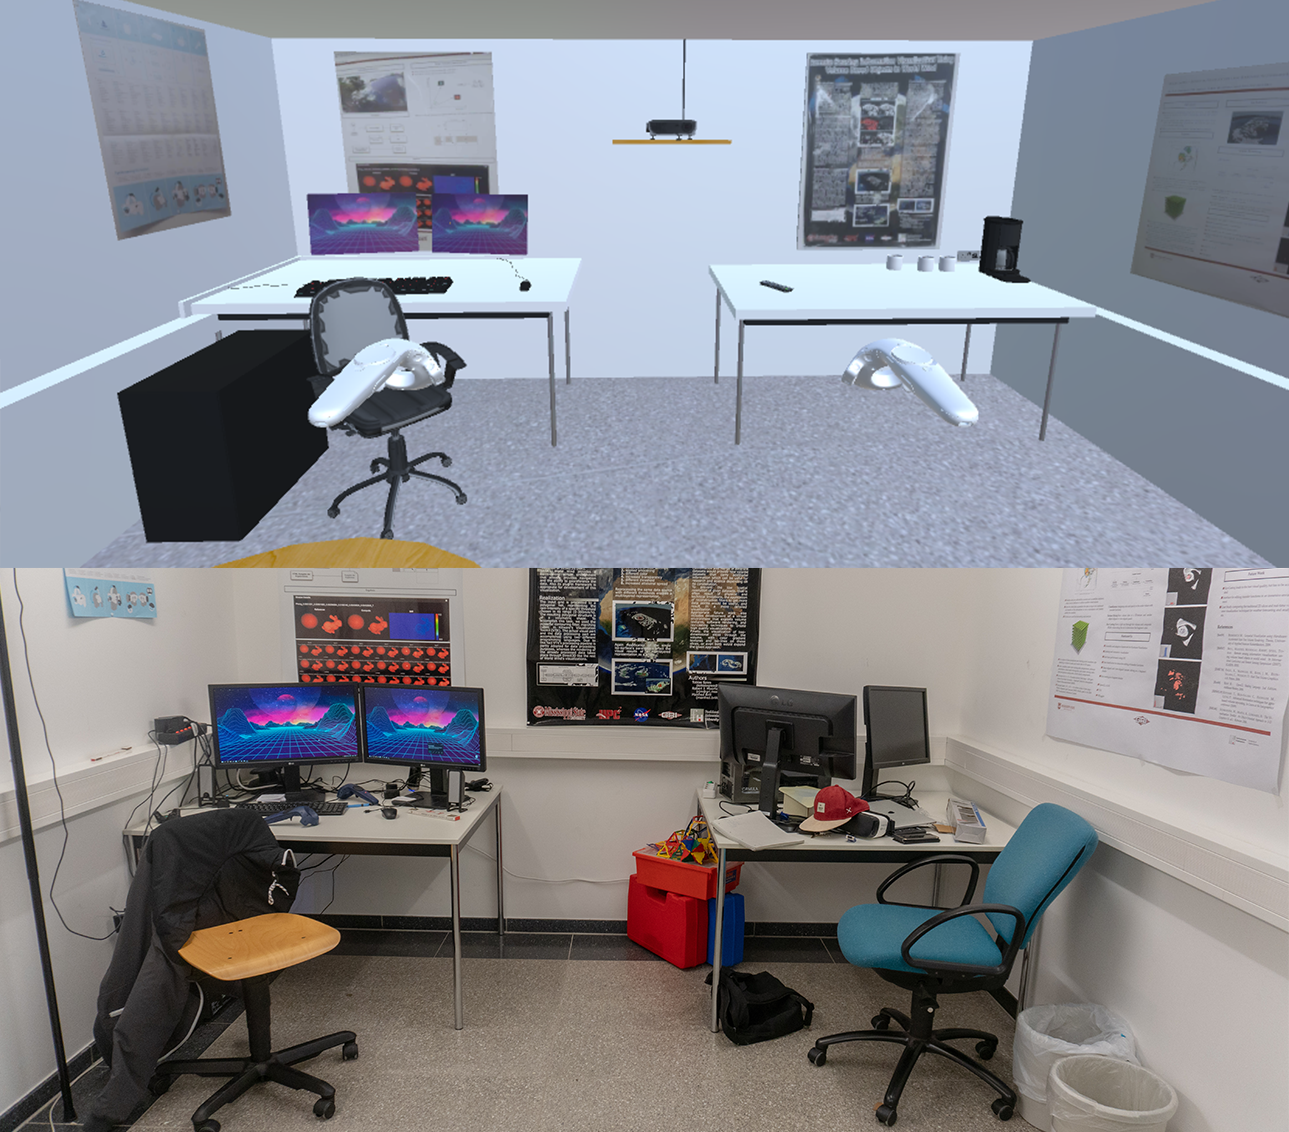
\includegraphics[width=1\textwidth]{images/labor/labor_vgl.png}
	\caption{Vergleich reales Labor - virtuelles Labor}
	\label{img:labor}
\end{figure}